%
% !TEX root = babylm_accuracy_morph_short.tex
%
\pdfoutput=1
\documentclass[11pt]{article}

\usepackage[review]{acl}
\usepackage{times}
\usepackage{latexsym}
\usepackage[T1]{fontenc}
\usepackage[utf8]{inputenc}
\usepackage{microtype}
\usepackage{amsmath}
\usepackage{booktabs}
\usepackage{colortbl}
\usepackage{graphicx}
\usepackage{tikz}
\usetikzlibrary{arrows.meta,positioning}
\usepackage[breaklinks]{hyperref}

\urlstyle{same}
\definecolor{tablegray}{gray}{0.93}

\title{Can Masking Words the Model Gets Wrong Improve Small Language Model Pretraining? A BabyLM Shared Task Experiment}

\author{
  First Author \\
  Affiliation \\
  \texttt{email@example.com}
}

\begin{document}
\maketitle

\begin{abstract}
Adaptive masking can improve masked language model pretraining, but it remains unclear which online feedback signals are reliable under strict small-data controls.
This paper studies a simple research question: can a model learn more by masking words it has repeatedly predicted incorrectly?
The question is tested in BabyLM Strict-Small by keeping the dataset, tokenizer, architecture, optimizer, schedule, training length, replacement policy, and total 15\% mask rate fixed, changing only which token positions are selected for prediction.
The paper introduces Accuracy-Morph, which tracks token and character-trigram exposure and top-1 prediction errors, then allocates a small portion of the mask budget to patterns repeatedly predicted incorrectly.
Three random MLM baseline seeds are available overall; in the matched seeds 1 and 2, Accuracy-Morph improves validation MLM loss by $-0.0155 \pm 0.0051$ and Entity Tracking by $+5.51 \pm 3.27$.
This suggests that correctness-smoothed feedback is promising, although the matched two-seed method comparison is not enough to establish a robust method.
\end{abstract}

\section{Introduction}

Masked language model (MLM) pretraining uses only a subset of tokens as direct prediction targets.
In large-scale pretraining, random masking may be enough because the model sees enormous numbers of masked examples.
In BabyLM-style small-data pretraining, however, the prediction budget is sharply limited: if only 15\% of tokens are masked, the choice of which tokens receive loss may matter.
This motivates a narrower question: under fixed small-LM controls, which online signal should decide what gets masked?

The goal is not to introduce adaptive masking as a new paradigm.
Instead, the study asks whether a simple online correctness signal can improve mask selection when the dataset, tokenizer, model architecture, optimizer, training schedule, training length, BERT-style replacement policy, and total 15\% mask rate are all held fixed.

\paragraph{RQ.}
\textbf{Can small language models learn more by masking words they repeatedly get wrong?}
The RQ is deliberately narrow: it asks whether one low-cost correctness signal can improve which positions are selected for prediction under a fixed 15\% MLM budget, not whether adaptive masking is new or whether changing the broader BabyLM recipe improves performance.

Accuracy-Morph is a correctness-smoothed adaptive masking policy.
During pretraining, it records how often each masked token string and each character trigram has been observed, and how often the model's top-1 prediction was wrong.
After a random warmup, a small part of the mask budget is allocated to token and trigram patterns with high smoothed error rates.
The method therefore targets repeated prediction failure rather than one-off high-loss events.

The contribution is a focused signal-level pilot.
Under a fixed MLM prediction budget, Accuracy-Morph is the operational test of the RQ: it tests whether repeated top-1 prediction failure is a useful online signal for selecting future masked positions.
Across the two matched method seeds, it improves validation MLM loss and gives the clearest official diagnostic movement on Entity Tracking.
At the same time, BLiMP and BLiMP Supplement are flat or slightly lower, so the matched two-seed result is not enough for a robust positive claim.
Accuracy-Morph is therefore treated as exploratory evidence that correctness-smoothed feedback is a promising adaptive masking signal.

\section{Related Work}

BabyLM evaluates sample-efficient pretraining from limited, developmentally motivated corpora \citep{warstadt2023babylm,hu2024babylm,choshen2026babylm}.
Strong BabyLM approaches often modify architecture, objective, attention pattern, data curation, or optimization \citep{charpentier2024gptbert,yu2024antlm,haller2025sample,kosmopoulou2025masked}.
The question here is narrower: can target selection alone improve an otherwise unchanged MLM?

Prior masking work shows that prediction targets need not be uniform.
Task-guided masking selects tokens useful for downstream transfer \citep{gu2020train}, while informative masking estimates which tokens provide useful unsupervised signal \citep{sadeq2022informask}.
Curriculum masking changes target difficulty over training \citep{lee2022efficient}; learned or self-evolving masking policies adapt the pretraining objective itself \citep{yang2023learning,zhong2023self}; and difference-masking chooses targets for continued pretraining from domain contrast \citep{wilf2023difference}.
These studies motivate the central premise that what gets masked matters.
They also differ from the present setting in important ways: several use task information, auxiliary scoring models, explicit domain contrast, or broader changes to the pretraining recipe.

The closest prior work is BabyLM adaptive MLM, which changes masking probabilities according to model predictability and uses subtoken information to improve generalization \citep{edman2025mask}.
That work is the most direct precedent because it is also BabyLM-specific, model-aware, and concerned with making MLM prediction targets more useful under small-data constraints.
The present work is complementary rather than a claim of novelty for adaptive masking: it isolates a smaller signal-level question.
The corpus, tokenizer, model, optimizer, schedule, training length, replacement policy, and total 15\% mask rate are held fixed.
Under those controls, the experiment tests whether a cheap online signal is useful for selecting a small subset of future MLM targets.
That signal is smoothed top-1 prediction correctness over token strings and character trigrams.

The main distinction is therefore not that Accuracy-Morph is adaptive, but how little it asks from the rest of the training setup.
Unlike task-guided or domain-contrast masking, it uses no labels, external data, or external scorer.
Unlike methods that treat a token as difficult after a single high-loss event, it requires repeated prediction failure before increasing masking pressure.
Unlike approaches that change the tokenizer or add linguistic analyzers, its subtoken component is only a character-trigram proxy for surface-form regularities.
This makes the experiment a controlled test of one online feedback signal rather than a new full pretraining recipe.

\section{Method}

\subsection{Controlled Masking-Only Setup}

All approaches preserve the same total MLM mask rate of 15\%.
They differ only in how valid non-special, non-padding token positions are selected for prediction.
After selection, every approach applies the same BERT-style replacement policy: 80\% of selected positions are replaced by \texttt{[MASK]}, 10\% by a random vocabulary token, and 10\% are left unchanged.
Labels for unmasked positions are set to \texttt{-100}.
If an adaptive source cannot provide enough eligible positions, the remaining budget is filled uniformly at random.
No validation or test examples are used to update adaptive statistics.

\subsection{Accuracy-Morph}

Accuracy-Morph is a correctness-smoothed adaptive masking policy that uses online token and character-trigram statistics to allocate a small portion of the MLM mask budget to candidates the model repeatedly predicts incorrectly.
The method comes from a failure mode in raw difficulty masking: a single high-loss event can reflect noise, rare names, tokenization artifacts, or early-training instability.
Accuracy-Morph instead treats difficulty as repeated prediction failure.
It was motivated by diagnosing raw-loss adaptive masking as too reactive, then replacing raw loss with a smoothed estimate of repeated top-1 prediction failure.
It asks whether a token or surface pattern has been observed as an MLM target before, and whether the model has repeatedly failed to place the correct label at the top of its prediction distribution.

For every masked training token, the model's top-1 prediction is compared with the true MLM label.
The collator maintains exposure and error counts for two feature types: the full token string and character trigrams extracted from the normalized token string.
If the model predicts the true label at rank 1, only the exposure count is incremented.
If the top-1 prediction is different from the true label, both exposure and wrong-prediction counts are incremented.
These updates are made only for positions already selected by the MLM objective, so the adaptive policy learns from the same prediction events that train the model.
For a token or trigram feature $x$, the score is
\begin{equation}
s(x) = \frac{\mathrm{wrong}(x) + 0.5}{\mathrm{seen}(x) + 1.0}.
\end{equation}
For token-guided masking, candidate positions are scored by their token-string score.
For morph-guided masking, candidate positions are scored by the mean score of their character trigrams.

\begin{figure}[t]
\centering
\scriptsize
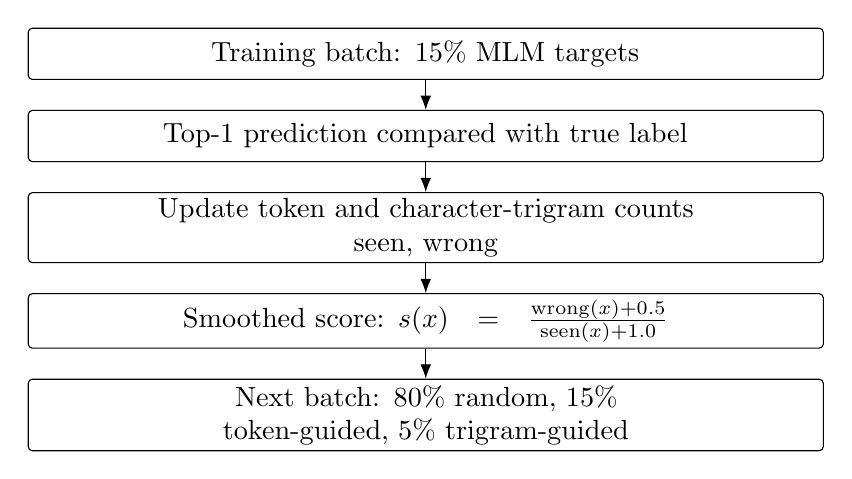
\begin{tikzpicture}[
  node distance=3.8mm,
  box/.style={draw, rounded corners=1.5pt, align=center, inner sep=2.2pt, minimum height=6.5mm, text width=0.82\columnwidth},
  arrow/.style={-{Latex[length=1.8mm]}, line width=0.35pt}
]
\node[box] (batch) {Training batch: 15\% MLM targets};
\node[box, below=of batch] (pred) {Top-1 prediction compared with true label};
\node[box, below=of pred] (counts) {Update token and character-trigram counts\\seen, wrong};
\node[box, below=of counts] (score) {Smoothed score: $s(x)=\frac{\mathrm{wrong}(x)+0.5}{\mathrm{seen}(x)+1.0}$};
\node[box, below=of score] (mix) {Next batch: 80\% random, 15\% token-guided, 5\% trigram-guided};
\draw[arrow] (batch) -- (pred);
\draw[arrow] (pred) -- (counts);
\draw[arrow] (counts) -- (score);
\draw[arrow] (score) -- (mix);
\end{tikzpicture}
\caption{Accuracy-Morph uses only training-time MLM prediction events. Masked tokens update token and character-trigram exposure/error counts; smoothed error scores then guide a small portion of the next mask budget while the total mask rate remains fixed at 15\%.}
\label{fig:accuracy_morph_loop}
\end{figure}

As a hands-on example, suppose a training batch contains the sentence fragment ``the child is running outside,'' and the random warmup masks \textit{running}.
The true label is \textit{running}, but the model's top prediction is \textit{walking}.
The update records one exposure and one error for the token string \textit{running}.
It also records one exposure and one error for the character trigrams extracted from the normalized surface form, such as \textit{run}, \textit{unn}, \textit{nni}, \textit{nin}, and \textit{ing}.
If later batches mask \textit{running} three more times and the model is correct once and wrong twice, the stored token counts become $\mathrm{seen}(\textit{running})=4$ and $\mathrm{wrong}(\textit{running})=3$.
The token score is then $(3+0.5)/(4+1)=0.70$.
A different token seen four times and missed once scores $(1+0.5)/(4+1)=0.30$, so a later \textit{running} position is more likely to be chosen for the token-guided part of the mask budget.

The character-trigram component gives the policy a small amount of surface-form generalization.
For example, a later sentence may contain \textit{runner} or \textit{running} in an unmasked candidate position.
Even if \textit{runner} has rarely been masked as a full token, it shares trigrams such as \textit{run} and \textit{unn} with previous high-error events.
The morph-guided score averages the smoothed error estimates of those trigrams, so related forms can receive some adaptive pressure without changing the tokenizer, adding external morphology, or increasing the total number of masks.
The term ``Morph'' is used descriptively: character trigrams share difficulty across surface forms without changing the tokenizer or adding a morphological analyzer.

The smoothing constants prevent rare one-off observations from dominating selection.
Accuracy-Morph instead requires repeated top-1 prediction failure before a token or subtoken pattern becomes attractive.
Unseen features start at $0.5$ rather than an extreme value; as evidence accumulates, the score moves toward its empirical error rate.

The policy uses a 30\% random warmup.
After warmup, the intended mask mixture is 80\% random masks, 15\% token-correctness-guided masks, and 5\% character-trigram-correctness-guided masks.
For a sequence with 100 eligible tokens, the collator still selects about 15 total MLM targets.
After warmup, this corresponds roughly to 12 random targets, 2 token-score targets, and 1 trigram-score target, with rounding handled per batch.
If the token or trigram scorer cannot supply enough non-duplicate eligible positions, the missing positions are filled randomly.
The total mask rate remains fixed at 15\%, so Accuracy-Morph changes only which positions are predicted, not how many predictions the model receives.

\section{Experimental Setup}

\paragraph{Data and Controls.}
The experiments use BabyLM 2026 Strict-Small: 10M words from BNC spoken, CHILDES, Gutenberg, OpenSubtitles, Simple Wikipedia, and Switchboard.\footnote{Dataset: \url{https://huggingface.co/datasets/BabyLM-community/BabyLM-2026-Strict-Small}.}
All approaches share the same split, \texttt{bert-base-uncased} tokenizer, compact BERT-style MLM, optimizer, schedule, training length, replacement policy, and 15\% mask rate; only mask selection changes.

\paragraph{Model and Training.}
The model has hidden size 256, 4 layers, 4 attention heads, intermediate size 1024, and maximum position embeddings 512.
Training uses maximum sequence length 128, batch size 64, 10{,}000 steps, learning rate $5 \times 10^{-4}$, weight decay 0.01, gradient clipping at 1.0, and warmup fraction 0.06.
Runs were executed on a single NVIDIA RTX A6000 GPU.
The final checkpoint and prepared prediction bundle are available on Hugging Face.\footnote{\url{https://huggingface.co/alonsopg/babylm-2026-accuracy-morph-strict-small}.}
Three random MLM baseline seeds were trained overall.
Accuracy-Morph has two matched seeds, so paired deltas use seeds 1 and 2; the third random seed is baseline context only.

\paragraph{Evaluation.}
The primary metric is validation MLM loss after 10k steps.\footnote{Local validation uses 2{,}000 held-out examples and 40 evaluation batches with the same MLM objective used during training.}
Available BabyLM strict diagnostics are also run.\footnote{Evaluation code: \url{https://github.com/babylm-org/babylm-eval}. Full filtered EWoK was run after obtaining dataset access. AoA is not reported as a complete metric because the official strict-small pipeline expects a checkpoint series, while only the final checkpoint was retained.}
BLiMP and Supplement test minimal-pair acceptability; EWoK tests world-knowledge contrasts; Entity Tracking tests discourse-entity state; COMPS tests compositionality; and Reading compares surprisal with eye-tracking and self-paced reading.
Lower is better for validation loss; higher is better for diagnostics.

\begin{table*}[t]
\centering
\fontsize{8.0}{8.7}\selectfont
\setlength{\tabcolsep}{2.4pt}
\renewcommand{\arraystretch}{1.0}
\begin{tabular}{@{}l c r r r r r r r r@{}}
\toprule
\textbf{Approach} & \textbf{Matched Seeds} & \textbf{Val. Loss} & \textbf{BLiMP} & \textbf{Sup.} & \textbf{EWoK} & \textbf{Entity} & \textbf{COMPS} & \textbf{Eye} & \textbf{SPR} \\
\midrule
\rowcolor{tablegray}
Random MLM & 1--2 & $3.0871$ & \textbf{62.79} & \textbf{55.86} & -- & $16.77$ & \textbf{50.31} & $1.55$ & $2.16$ \\
Accuracy-Morph & 1--2 & \textbf{3.0715} & $62.71$ & $55.60$ & $49.79$ & \textbf{22.28} & $50.30$ & \textbf{1.93} & \textbf{2.34} \\
\midrule
\rowcolor{tablegray}
Paired delta & 1--2 & \textbf{$-0.0155$} & $-0.08$ & $-0.26$ & -- & \textbf{$+5.51$} & $-0.00$ & \textbf{$+0.38$} & \textbf{$+0.19$} \\
\bottomrule
\end{tabular}
\caption{Matched-seed comparison over seeds 1 and 2. Three random MLM seeds were trained overall, but Accuracy-Morph currently has two matched seeds, so deltas use only those seeds. EWoK is reported for the final Accuracy-Morph checkpoint only; matched Random EWoK was not available, so no paired EWoK delta is reported. Lower is better for validation loss; higher is better for diagnostics.}
\label{tab:main-accuracy-morph}
\end{table*}

\section{Results}

Table~\ref{tab:main-accuracy-morph} shows the main result.
The results answer the RQ cautiously rather than conclusively.
Accuracy-Morph improves matched validation loss in both available seeds, with mean paired change $-0.0155 \pm 0.0051$.
The absolute improvement is small, but it is consistent across the two matched method seeds.

The official diagnostics are mixed.
The clearest movement is Entity Tracking: Accuracy-Morph improves the matched mean from 16.77 to 22.28, a paired gain of $+5.51 \pm 3.27$.
Reading diagnostics also improve modestly, with $+0.38$ on eye-tracking and $+0.19$ on self-paced reading.
BLiMP and BLiMP Supplement are slightly lower, and COMPS is essentially unchanged.
Full filtered EWoK for the final Accuracy-Morph checkpoint is near chance at 49.79 average accuracy, so the result is best viewed as pilot evidence rather than a broad official-evaluation win.

\section{Discussion and Limitations}

Returning to the RQ, the current answer is a qualified yes.
Smoothed top-1 prediction correctness appears useful in this controlled pilot because Accuracy-Morph improves matched validation loss in both available seeds and gives the clearest diagnostic gain on Entity Tracking.
However, the evidence does not support a stronger claim that the method is robust or broadly improves BabyLM evaluation: the validation-loss gain is small, BLiMP and Supplement are slightly lower, COMPS is unchanged, and EWoK remains near chance for the final checkpoint.
The most defensible interpretation is therefore signal-level rather than method-final: adaptive masking may benefit from repeated prediction-failure estimates, but the finding still needs confirmation.

The practical takeaways are that repeated top-1 prediction failure is more stable than one-off high-loss events, most masks should remain random to preserve broad corpus coverage, and character trigrams provide cheap surface-form transfer, for example between \textit{running} and \textit{runner}.
Thus Accuracy-Morph is intentionally conservative: it reserves a small part of the prediction budget for targets with accumulated evidence of being difficult for the current model.
The Entity Tracking gain suggests that this pressure may affect recurring lexical or discourse items, although this mechanism is not proven here.

Future work should prioritize a third matched seed, direct comparison to prior BabyLM adaptive MLM, token-only versus trigram-only ablations, analysis of selected tokens and trigrams, rare-token or morphology-focused slices, and difficulty-band filtering to avoid noisy or unlearnable highest-error items.
Future runs should also save the full checkpoint series for complete AoA evaluation.
No statistical significance claim is made from two matched seeds.
This work also does not aim to compete with BabyLM approaches that change the model family, objective, data, or training recipe; its purpose is narrower, isolating mask selection as the only intervention.

\section*{Ethics Statement}

This work changes which tokens receive prediction loss, not which documents are used.
The training corpus is fixed across conditions, so the method does not add or remove domains, speakers, or documents.
However, adaptive masking may shift training signal across lexical, morphological, or discourse patterns.
Future work should examine whether such shifts affect linguistic phenomena or data domains unevenly.

\bibliography{babylm-sketchselect-references}

\end{document}
